\documentclass[12pt, a4paper]{article}
\title{Homework 3: Solvers}
\author{Christopher Klammer \\ \small\texttt{cklammer@andrew.cmu.edu}}

% A pretty common set of packages
\usepackage[margin=2.5cm]{geometry}
\usepackage[T1]{fontenc}
\usepackage{graphicx}
\usepackage{amssymb}
\usepackage{amsmath}
\usepackage{bm}
\usepackage{color}
\usepackage{float}
\usepackage{bm}
\usepackage{physics}
\usepackage{subcaption}

\begin{document}
\maketitle
\section{Linear SLAM}
\subsection{Measurement Function}
\subsubsection{Odometry Measurement}
\textbf{The odometry measurement should just be the vector from the pose at time $t$ to the pose at time $t+1$}
$$h_{o}(\vectorbold{r^t}, \vectorbold{r^{t+1}}) = 
\begin{bmatrix} r^{t+1}_x - r^t_x  & r^{t+1}_y - r^t_y \end{bmatrix}^T$$ 

$$H_{o} = \begin{bmatrix}
    \frac{\partial r^{t+1}_x - r^t_x}{\partial r^t_x} & \frac{r^{t+1}_x - r^t_x}{\partial r^t_y}& \frac{\partial r^{t+1}_x - r^t_x}{\partial r^{t+1}_{x}} & \frac{\partial r^{t+1}_x - r^t_x}{\partial r_y^{t+1}} \\
    \frac{\partial r^{t+1}_y - r^t_y}{\partial r^t_x} & \frac{\partial r^{t+1}_y - r^t_y}{\partial r^t_y}& \frac{\partial r^{t+1}_y - r^t_y}{\partial r^{t+1}_{x}} & \frac{\partial r^{t+1}_y - r^t_y}{\partial r_y^{t+1}}
\end{bmatrix}$$

$$H_{o} = \begin{bmatrix}
    -1 & 0 & 1 & 0 \\
    0 & -1 & 0 & 1
\end{bmatrix}$$

\subsubsection{Landmark Measurement}
\textbf{This will be extremely similar, just find the vector from the robot's position to the landmark}
$$h_{l}(\vectorbold{r^t}, \vectorbold{l^k}) = 
\begin{bmatrix} l^k_x - r^t_x  & l^k_y - r^t_y \end{bmatrix}^T$$


$$H_l = \begin{bmatrix}
    \frac{\partial l^k_x - r^t_x}{\partial r^t_x} & \frac{\partial l^k_x - r^t_x}{\partial r^t_y} & \frac{\partial l^k_x - r^t_x}{\partial l^k_x} & \frac{\partial l^k_x - r^t_x}{\partial l^k_y} \\
    \frac{\partial l^k_y - r^t_y }{\partial r^t_x} & \frac{\partial l^k_y - r^t_y }{\partial r^t_y} & \frac{\partial l^k_y - r^t_y }{\partial l^k_x} & \frac{\partial l^k_y - r^t_y }{\partial l^k_y}
\end{bmatrix}$$

$$H_l = \begin{bmatrix}
    -1 & 0 & 1 & 0 \\
    0  & -1 & 0 & -1
\end{bmatrix}$$

\subsection{Solvers and Sparsity}
\subsubsection{2D Linear Data}
\textbf{Timing:}

\begin{tabular}{|c | c | c | c | c|}
    \hline
    \textbf{PInv} & \textbf{LU} & \textbf{LU COLAMD} & \textbf{QR} & \textbf{QR COLAMD} \\
    \hline
    \hline
    4.900 sec & 0.073 sec & 0.186 sec & 1.074 sec & 1.113 sec \\
    \hline
\end{tabular}

\begin{figure}
    \center
    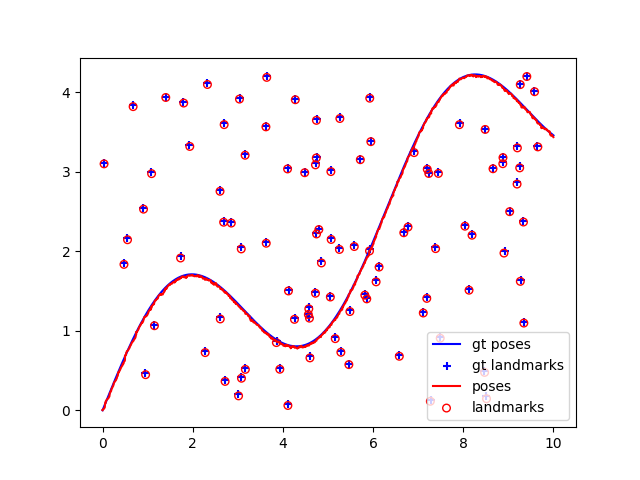
\includegraphics[width=0.75\textwidth]{linear_results/PInv_Traj.png}
    \caption{Trajectory for PInv Solver}
\end{figure}

\begin{figure}
    \center
    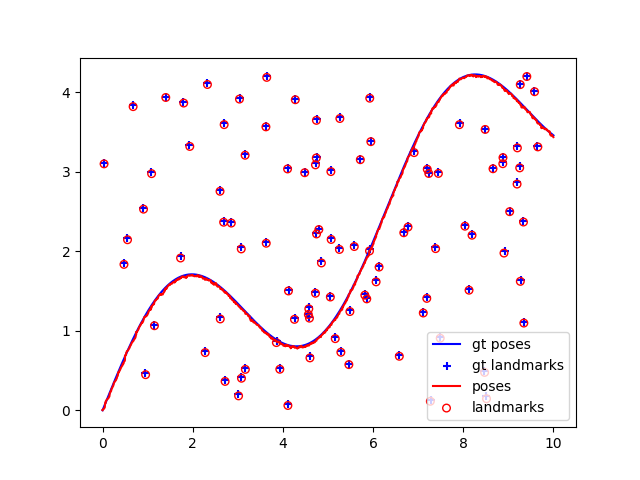
\includegraphics[width=0.75\textwidth]{linear_results/LU_Factor_Traj.png}
    \caption{Trajectory for LU Solver}
\end{figure}

\begin{figure}
    \center
    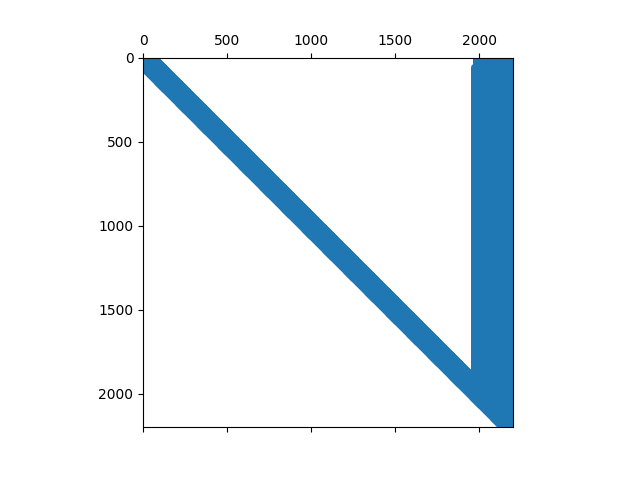
\includegraphics[width=0.75\textwidth]{linear_results/LU_Factor_Sparsity.png}
    \caption{Sparsity for LU Solver}
\end{figure}

\begin{figure}
    \center
    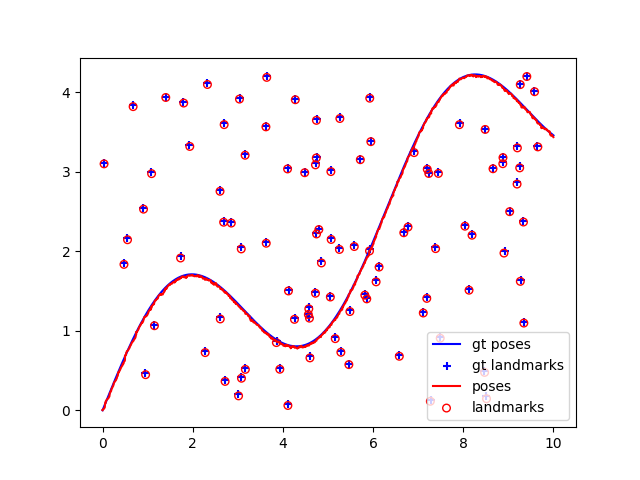
\includegraphics[width=0.75\textwidth]{linear_results/LU_COLAMD_Traj.png}
    \caption{Trajectory for LU COLAMD Solver}
\end{figure}

\begin{figure}
    \center
    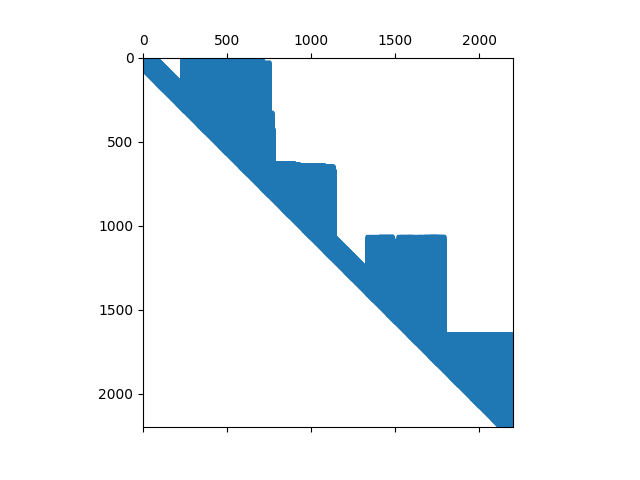
\includegraphics[width=0.75\textwidth]{linear_results/LU_COLAMD_Sparsity.png}
    \caption{Sparsity for LU COLAMD Solver}
\end{figure}

\begin{figure}
    \center
    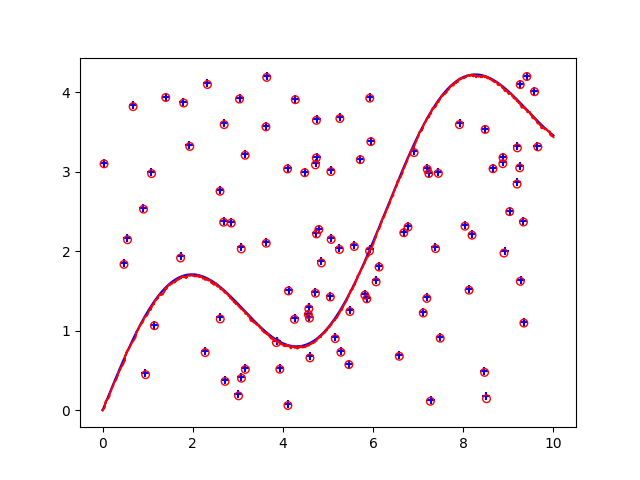
\includegraphics[width=0.75\textwidth]{linear_results/QR_Traj.png}
    \caption{Trajectory for QR Solver}
\end{figure}

\begin{figure}
    \center
    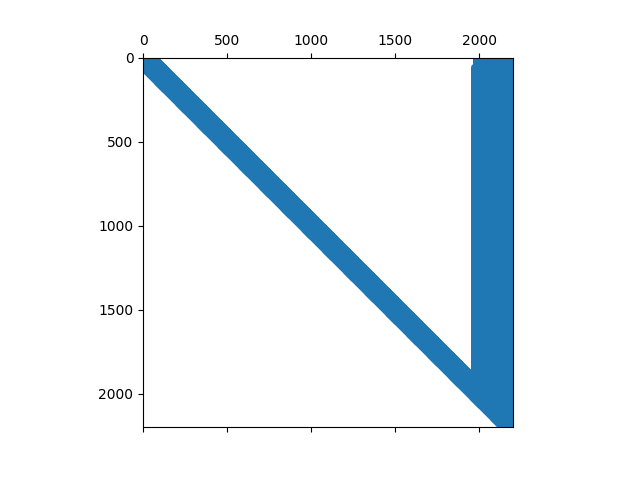
\includegraphics[width=0.75\textwidth]{linear_results/QR_Sparsity.png}
    \caption{Sparsity for QR Solver}
\end{figure}

\begin{figure}
    \center
    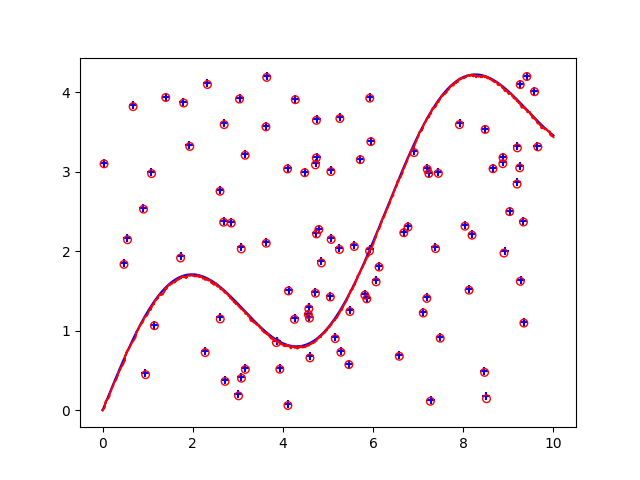
\includegraphics[width=0.75\textwidth]{linear_results/QR_COLAMD_Traj.png}
    \caption{Trajectory for QR COLMAD Solver}
\end{figure}

\begin{figure}
    \center
    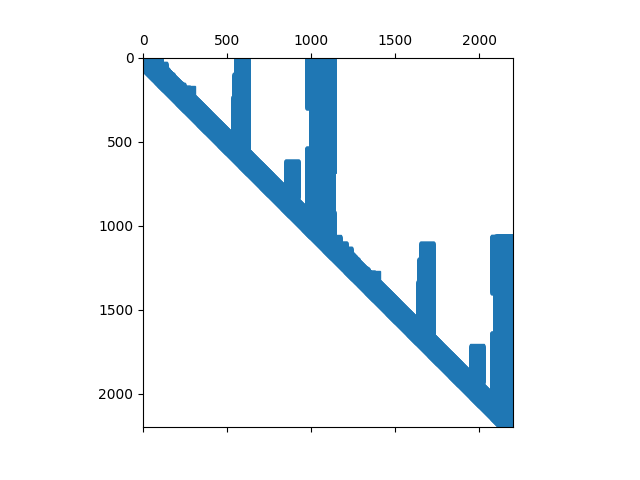
\includegraphics[width=0.75\textwidth]{linear_results/QR_COLAMD_Sparsity.png}
    \caption{Sparsity for QR COLMAD Solver}
\end{figure}

\clearpage
\subsubsection{2D Linear Discussion}
First off, we see here that the psuedo-inverse is the slowest, the LU solver is the fastest, and the QR solver is in the middle. We also see that the COLAMD methods do not cause any speedup.

In the case of a linear trajectory, we do not have any redundant observations. Each landmark that we see is relatively new and, since the trajectory is fairly linear, we see that our factorized matricies are sparse and close to diagonal. Since this is the case, we do not see performance increase by using the COLAMD ordering. In my opinion, it seems that no further sparsification can be gained with COLAMD so the reordering acts as an overhead making the performance worse.

\clearpage
\subsubsection{2D Linear Loop Data}
\textbf{Timing:}

\begin{tabular}{|c | c | c | c | c|}
    \hline
    \textbf{PInv} & \textbf{LU} & \textbf{LU COLAMD} & \textbf{QR} & \textbf{QR COLAMD} \\
    \hline
    \hline
    0.451 sec & 0.056 sec & 0.009 sec & 0.616 sec & 0.063 sec \\
    \hline
\end{tabular}

\begin{figure}
    \center
    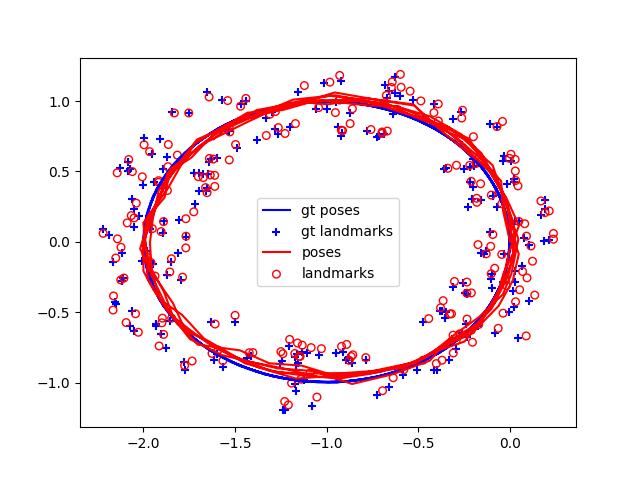
\includegraphics[width=0.75\textwidth]{linear_loop_results/loop_pinv.png}
    \caption{Trajectory for PInv Solver}
\end{figure}

\begin{figure}
    \center
    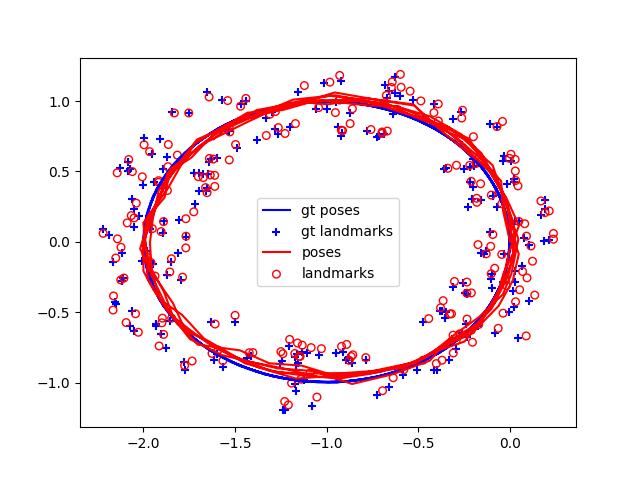
\includegraphics[width=0.75\textwidth]{linear_loop_results/loop_lu.png}
    \caption{Trajectory for LU Solver}
\end{figure}

\begin{figure}
    \center
    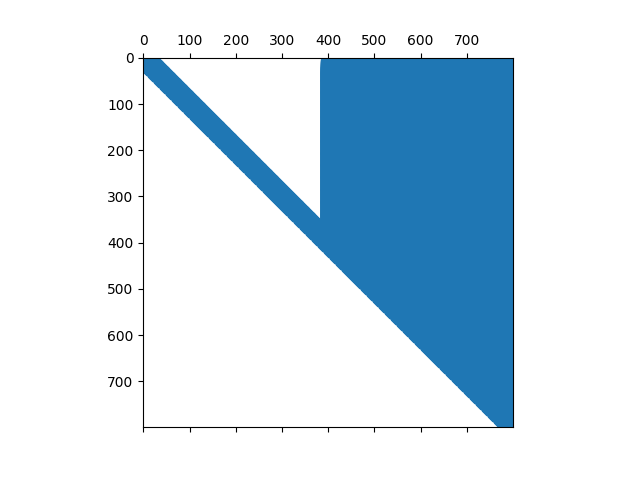
\includegraphics[width=0.75\textwidth]{linear_loop_results/lu_sparsity_loop.png}
    \caption{Sparsity for LU Solver}
\end{figure}

\begin{figure}
    \center
    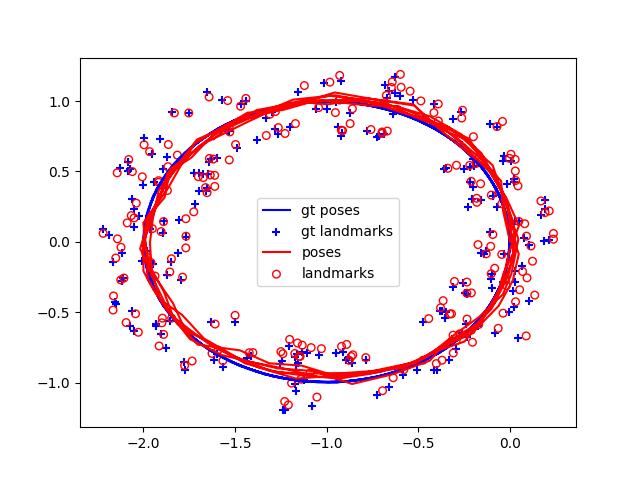
\includegraphics[width=0.75\textwidth]{linear_loop_results/lu_colamd.png}
    \caption{Trajectory for LU COLAMD Solver}
\end{figure}

\begin{figure}
    \center
    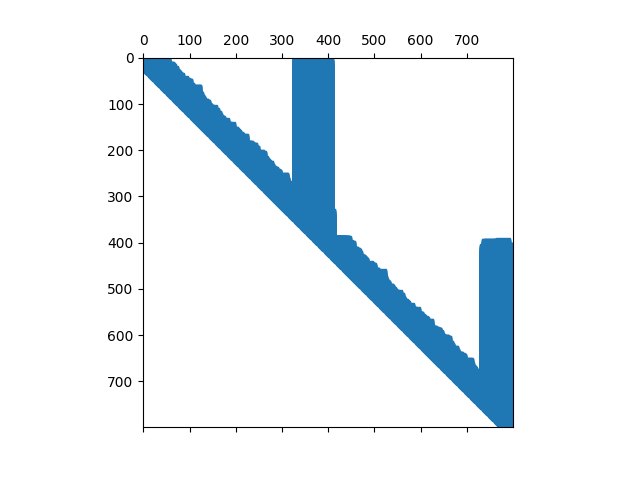
\includegraphics[width=0.75\textwidth]{linear_loop_results/lu_colamd_sparsity.png}
    \caption{Sparsity for LU COLAMD Solver}
\end{figure}

\begin{figure}
    \center
    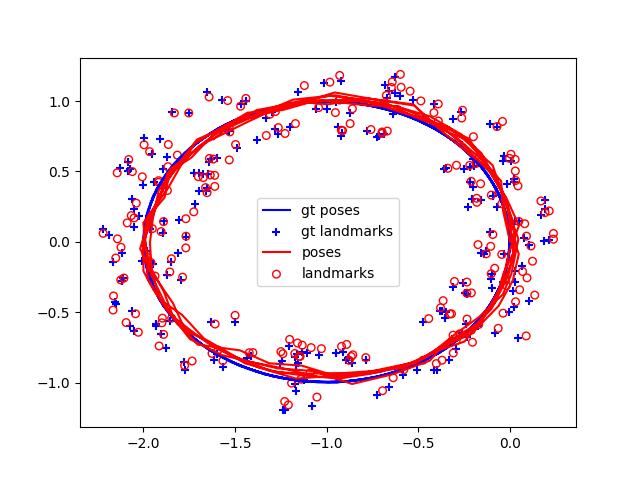
\includegraphics[width=0.75\textwidth]{linear_loop_results/loop_qr.png}
    \caption{Trajectory for QR Solver}
\end{figure}

\begin{figure}
    \center
    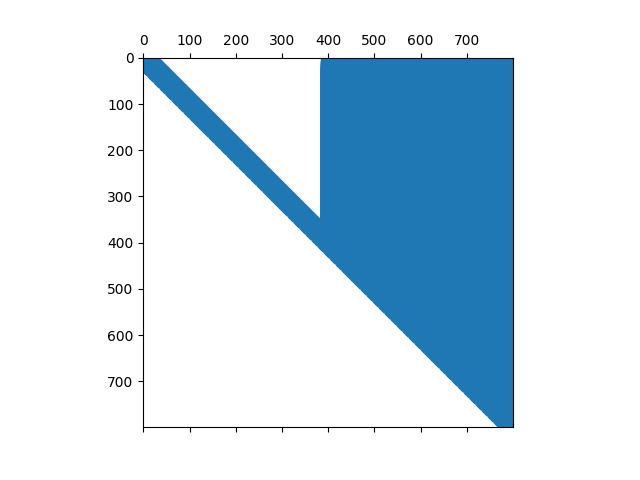
\includegraphics[width=0.75\textwidth]{linear_loop_results/qr_sparsity_loop.png}
    \caption{Sparsity for QR Solver}
\end{figure}

\begin{figure}
    \center
    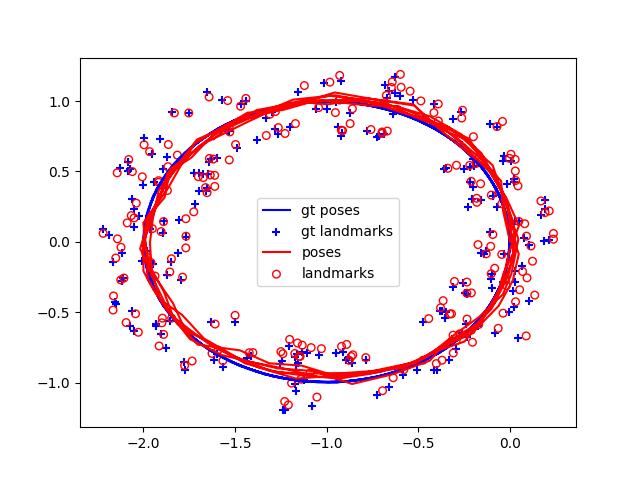
\includegraphics[width=0.75\textwidth]{linear_loop_results/qr_colamd.png}
    \caption{Trajectory for QR COLMAD Solver}
\end{figure}

\begin{figure}
    \center
    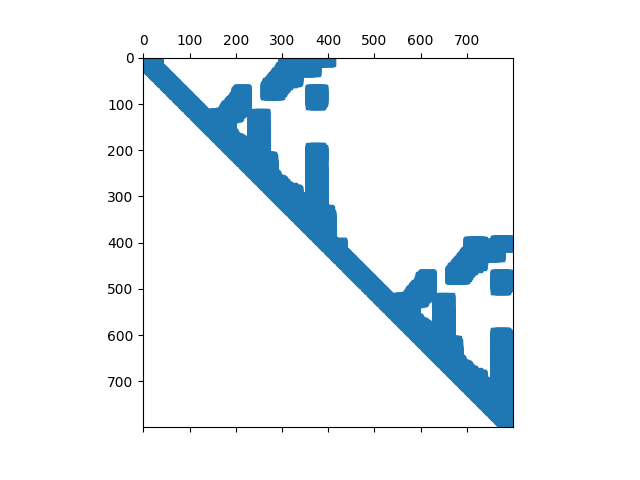
\includegraphics[width=0.75\textwidth]{linear_loop_results/qr_colamd_sparsity.png}
    \caption{Sparsity for QR COLMAD Solver}
\end{figure}

\clearpage
\subsubsection{2D Linear Loop Discussion}
In general, we see the same relative ordering in that the psuedo-inverse is the slowest, the LU solver is the quickest, and the QR solver is in the middle. However, in this case, we see that COLAMD offers massive speedups.


In this case, we appear to move in a loop where we visit the same landmarks multiple times and we also see similar odometry measurements as well because we are moving in the same loop. This creates a much more dense matrix, especially compared to the linear case.

Here, we see large speedups in performance when using the COLAMD ordering which helps sparsify the matrix by removing more redudant measurements. For example, seeing the same landmark from the same pose is probably not useful, we can essentially remove or generally combine these redundant rows in order to create a more sparse representation. 

\section{Non-Linear SLAM}
\subsection{Measurement Function}
\subsubsection{Landmark Measurement}
\textbf{Notation:}
$$dx = l_x^k - r_x^t$$
$$dy = l_y^k - r_y^t$$
\\
\textbf{Calculation:}
$$H_{l} = \begin{bmatrix}
    \frac{\partial \theta}{\partial r^t_x} & \frac{\partial \theta}{\partial r^t_y}& \frac{\partial \theta}{\partial l_x^k} & \frac{\partial \theta}{\partial l_y^k} \\
    \frac{\partial d}{\partial r^t_x} & \frac{\partial d}{\partial r^t_y}& \frac{\partial d}{\partial l_x^k} & \frac{\partial d}{\partial l_y^k}
\end{bmatrix}$$
\\
$$\frac{\partial \theta}{\partial r_x^t} = \frac{dx^2}{dx^2 + dy^2} * \frac{dy}{dx^2} = \frac{dy}{dx^2 + dy^2}$$

$$\frac{\partial \theta}{\partial r_y^t} = \frac{dx^2}{dx^2 + dy^2} * -\frac{dx}{dx^2} = -\frac{dx}{dx^2 + dy^2}$$

$$\frac{\partial \theta}{\partial l_x^k} = \frac{dx^2}{dx^2 + dy^2} * \frac{-dy}{dx^2} = -\frac{dy}{dx^2 + dy^2}$$

$$\frac{\partial \theta}{\partial l_y^k} = \frac{dx^2}{dx^2 + dy^2} * \frac{dx}{dx^2} = \frac{dx}{dx^2 + dy^2}$$

$$\frac{\partial d}{\partial r_x^t} = \frac{1}{2} * (dx^2 + dy^2)^{-\frac{1}{2}} * -2 * dx = \frac{-dx}{(dx^2 + dy^2)^{1/2}}$$

$$\frac{\partial d}{\partial r_y^t} = \frac{1}{2} * (dx^2 + dy^2)^{-\frac{1}{2}} * -2 * dy = \frac{-dy}{(dx^2 + dy^2)^{1/2}}$$

$$\frac{\partial d}{\partial l_x^k} = \frac{1}{2} * (dx^2 + dy^2)^{-\frac{1}{2}} * 2 * dx = \frac{dx}{(dx^2 + dy^2)^{1/2}}$$

$$\frac{\partial d}{\partial l_y^k} = \frac{1}{2} * (dx^2 + dy^2)^{-\frac{1}{2}} * 2 dy = \frac{dy}{(dx^2 + dy^2)^{1/2}}$$


$$H_{l} = \begin{bmatrix}
    \frac{dy}{dx^2 + dy^2} & \frac{-dx}{dx^2 + dy^2} & \frac{-dy}{dx^2 + dy^2} & \frac{dx}{dx^2 + dy^2} \\
    \frac{-dx}{(dx^2 + dy^2)^{1/2}} & \frac{-dy}{(dx^2 + dy^2)^{1/2}}& \frac{dx}{(dx^2 + dy^2)^{1/2}} & \frac{dy}{(dx^2 + dy^2)^{1/2}}
\end{bmatrix}$$

\end{document}